Occlusion-aware segmentation of deformable slender objects

Abstract

We propose an algorithm for detecting the topology of a deformable
slender object (DSO) in terms of its self intersections. The topology
refers to the order of self intersections that the DSO has with itself.
Based on the topology of the DSO, we can define the knot structure that
it forms. The proposed algorithm is important in robotic manipulaton of
DSO such as cables and ropes. Such deformable objects are oniquitous in
the natural environment, however, robotic manipulation still primarly
focuses on the rigid object assumption. The main challenge associated
with the manipulation of deformable objects come from the perception of
the object. The perception challenges arise from two key factor: (1) DSO
lack a fied shape, making their tracking and modelling complex, and (2)
self occlusions occur in certain configurations of the DLO, where parts
of the DLO obscure other sections. Traditional object detection methods
often rely on distinct geometric features that are effective for rigid
objects but fail when applied to deformable ones. To address these
challenges, we propose a DLO segmentation scheme that can segment DLOs
from a scene while also accounting for the order of self-occlusion. Our
approach involves a two-stage process: the first stage focuses on
segmentation, while the second stage resolves intersection ambiguities.
For segmentation, we propose to utilize a pre-trained segmentation
backbone and fine-tune it on a DLO-specific dataset to improve accuracy.
Once the intersection positions are identified, we hypothesize that the
order of intersection can be predicted by examining the change in RGB
values along the DLOs. Specifically, for the DLO on top, the RGB change
along its length will be minimal, whereas for the DLO beneath, a sharp
change in RGB values will be observed. We will validate this
self-occlusion-aware segmentation method using real-world images of
DLOs, evaluating both the accuracy of pixel segmentation and the correct
prediction of intersection order. The perception and segmentation of
deformable linear objects will allow for more natural interactions
between robots and DLO. This will have an impact in construction, cable
laying, medical applications etc. where robots can be used for DLO
manipulation. In particular, the order of self-occlusion is important
for knot-tying tasks that are common in medical suturing.

\begin{figure}
\centering
\pandocbounded{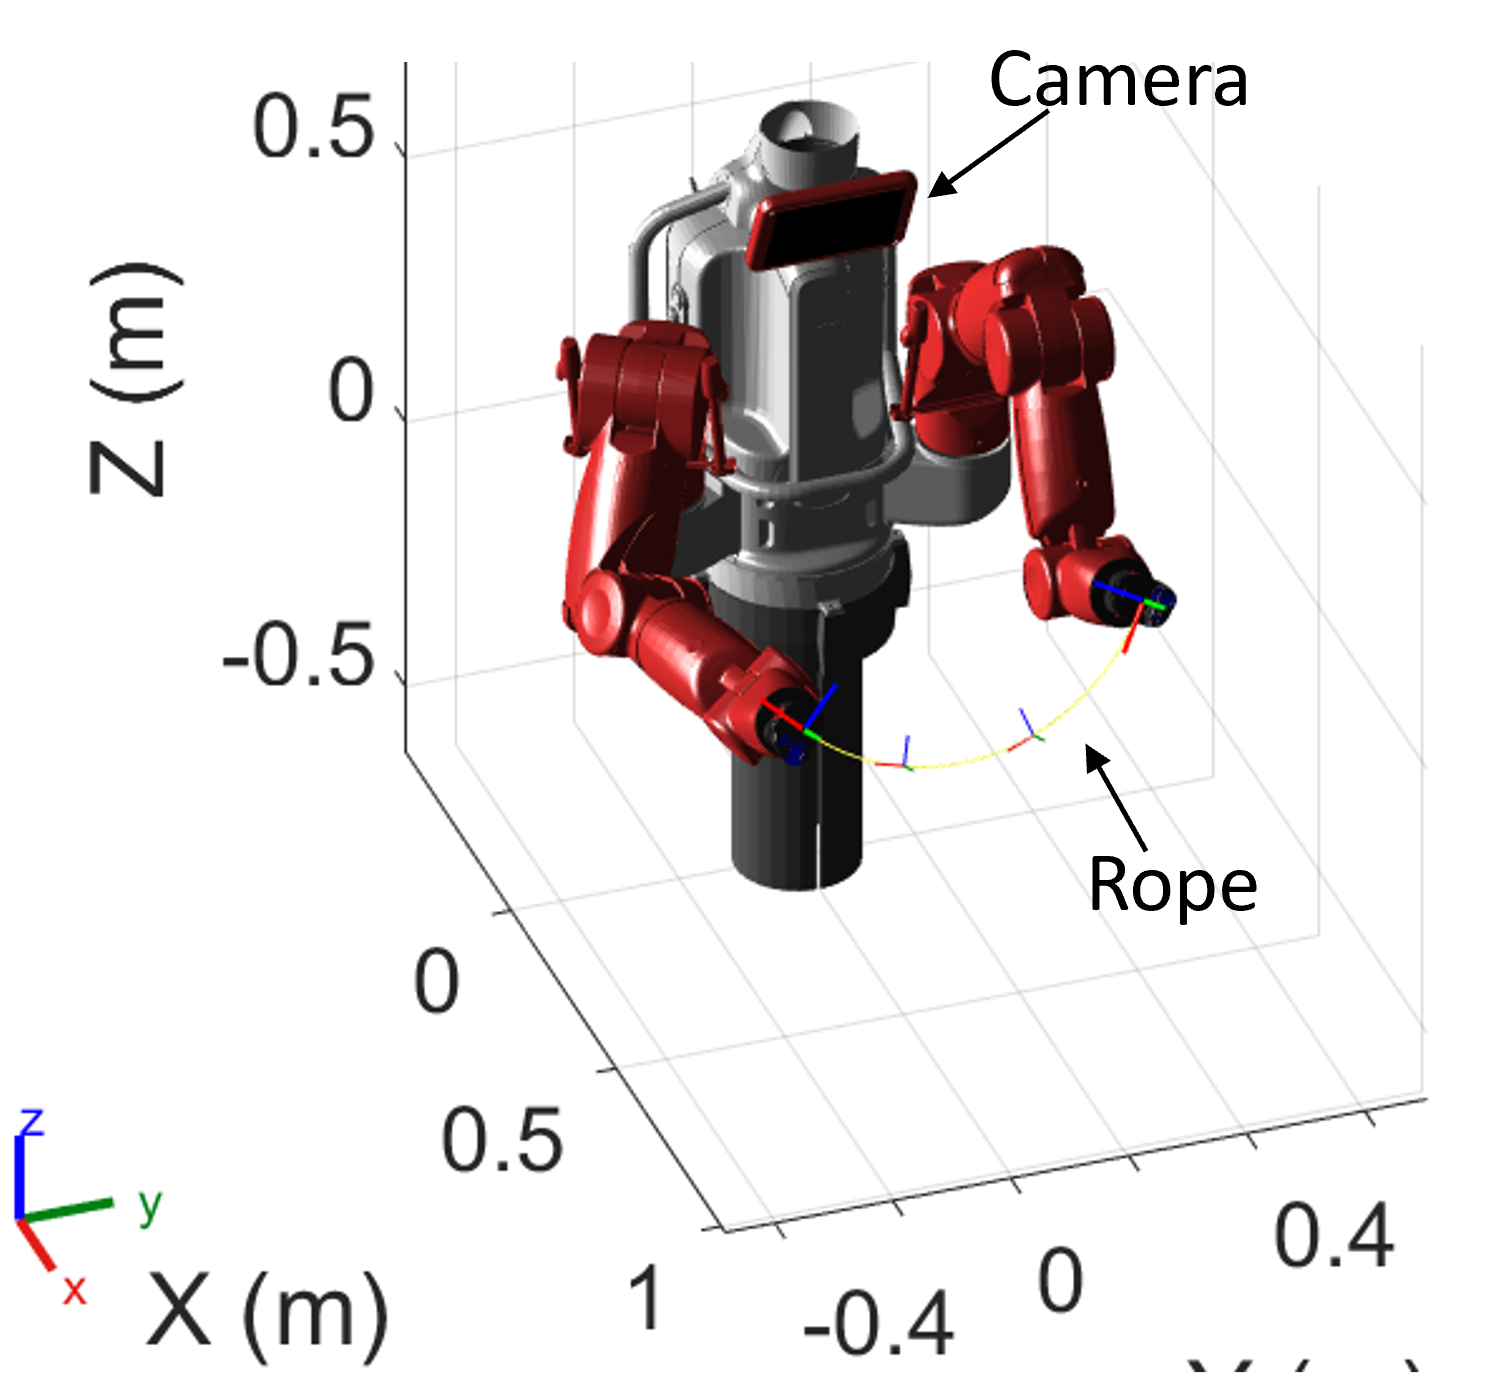
\includegraphics[keepaspectratio]{Abstract_picture.png}}
\caption{Image title}
\end{figure}

\textbf{Figure 1:} Vision based perception of DSO manipulation. During
manipulation, there may be different types of occlusions which the
proposed segmentation algorithm must be robust to.

Introduction

Defomable objects are all around us and humans are able to naturally
interact with them to accomplish various tasks that are not possible
with rigid objects. There are several challenges that limit the use of
robots for the manipulation of deformable objects. Unlike rigid objects,
deformable objects exhibit significant flexibility and elasticity that
make it difficult to model them effectively. Especially in the case of
active manipulation, the configuration of the object is dynamic and is
subject to change througout the manipulation. Without accurate
perception algorithms for deformable objects, robots would struggle to
find the current state of the deformable object and therefore cause
large errors in manipulation. Moreover, we need perception methods that
do not impose additional forces and moments on the deformable objects.
In this project, we propose to use a vision based method to percieve a
DSO that will be manipulated by a robot.

There are many different vision based methods that we can adopt to
develop algorithms for the perception of DSO in terms of the hardware
and the software. The different hardware solutions available to be used
are:

\subsubsection{Monocular camera}\label{monocular-camera}

Monocular cameras use a single sensor to percieve the environment around
them. They are widely used in robotic applications because they are
cheap and can provide a rich data about the environment. Monocular
cameras produce a 2D representation of the 3D world and because of this,
important depth information about the environment can be lost.

\begin{figure}
\centering
\pandocbounded{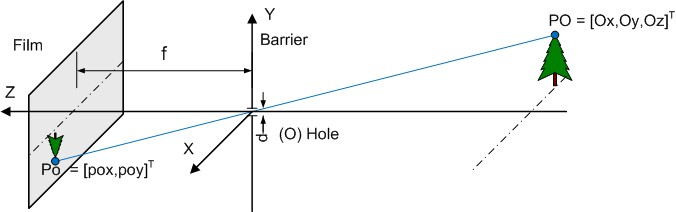
\includegraphics[keepaspectratio]{cam_model_fig41.jpg}}
\caption{alt text}
\end{figure}

\textbf{Figure 2:} Perspective projection model of a camera
\href{https://jordicenzano.name/front-test/2d-3d-paradigm-overview-2011/camera-model/}{{[}1{]}}

The image formation in a monocular camera can be modelled by the
perspective projection model which is given by: \[
\mathbf{p} = \frac{1}{Z}\begin{bmatrix}
f_x & 0 & c_x  \\
 0 & f_y & c_y \\ 
 0 &0& 1
 \end{bmatrix} \mathbf{P}
\]

Where \(\mathbf{p}\) is the position of the image on the image plane in
the homogenous coordinates, \(f_x\), \(f_y\), \(c_x\) and \(c_y\) are
the focal lengeths and the principle point coordinates respectievely.
Moreover, \(\mathbf{P}\) is the position of the object in the 3D scene.
It must be noted that a monocular camera produces a 2D projection of the
3D scene, therefore, it cannot measure directly the depth data that is
contained in the scene. There are however, algorithms to estimate the
depth information from monocular camera. The two main classes of
algorithms are: - Triangulation based methods: Ex. structure from
motion\{==cite==\} - Depth of field methods: Eg. depth from
defocus\{==cite==\}

A commonly used triangulation based technique is called structure from
motion. This involves capturing images from the same camera at two
different camera viewpoints, and using certain feature points that are
same on both pictures to reconstruct a 3D structure of the scene.

\begin{figure}
\centering
\pandocbounded{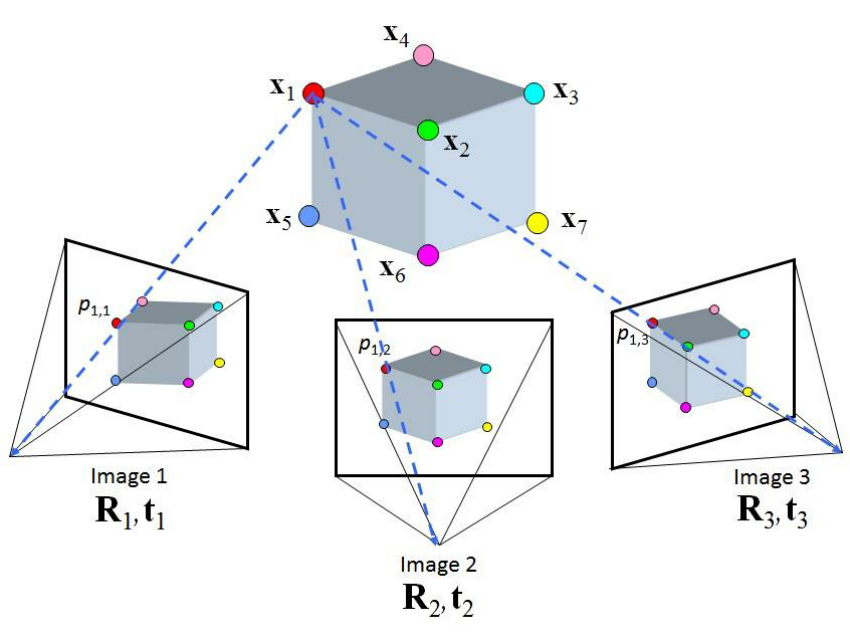
\includegraphics[keepaspectratio]{Structure-from-Motion-SfM-process-is-illustrated-The-structure-in-the.png}}
\caption{Structure from motion}
\end{figure}

\textbf{Figure 2:} By detecting the change of some feature points in the
image plane, the motion of the camera can be estimated. And using this,
the 3D representation of the scene can be obtained from pictures at
different viewpoints.\{==cite==\}

The key steps for estimating the 3d structure from a monocular camera
using structure from motion are:

\begin{itemize}
\tightlist
\item
  Capture multiple images from different viewpoints
\item
  Detect features such as corners that can be easily distinguished in
  different images
\item
  Match the detected features in one image to the other.
\item
  Estimate the motion of the camera between the two images. This can be
  done by solving the perspective-n-point problem.
\item
  The 3D position of the feature points are found by
  \{==triangulation==\}.
\end{itemize}

Another class of methods make use of the focus of the image produced to
estimate the depth information. A monocular camera has a limited range
of positions where it can capture a sharp image. This can be seen from:

\begin{figure}
\centering
\pandocbounded{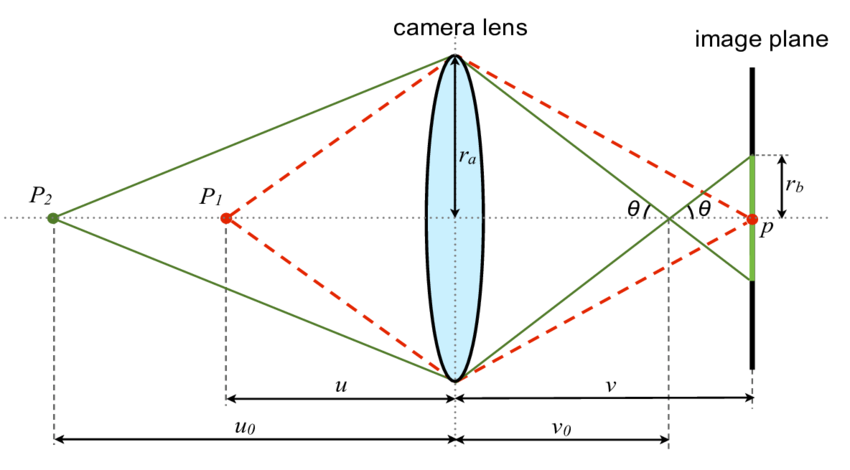
\includegraphics[keepaspectratio]{Depth-defocus-relationship-The-same-object-point-placed-at-different-distances-will-be.png}}
\caption{alt text}
\end{figure}

\textbf{Figure 2:} Objects at a distance \(u\) from the lens creates a
sharp image at the image plane. However, other objects will result in a
blurred
image.\href{https://www.researchgate.net/publication/273947737/figure/fig8/AS:650806445473802@1532175756521/Depth-defocus-relationship-The-same-object-point-placed-at-different-distances-will-be.png}{{[}2{]}}

USing the blur circle radius \(r_b\), we can have an estimate of the
depth by the equation:

{[}r\_b(z) = \frac{A(|z-z_f|)}{z}\frac{f}{z_f-f}{]} Where \(A\) is the
aperture size, \(f\) is the focal length, \(z_f\) is the distance to the
focal plane and finally \(z\) is the depth of the object. If we know the
blur circle radius, we can solve for \(z\) to estimate the depth from
defocus.

\subsubsection{Stereo camera}\label{stereo-camera}

Stereo cameras use a triangulation method to find the 3D data of the
scene. The major difference is that rather than using a single camera to
obtain multiple pictures of the scene, stereo cameras make use of
multiple cameras that have a known relative transformation to obtain
multiple images of the scene at the same time.

\begin{figure}
\centering
\pandocbounded{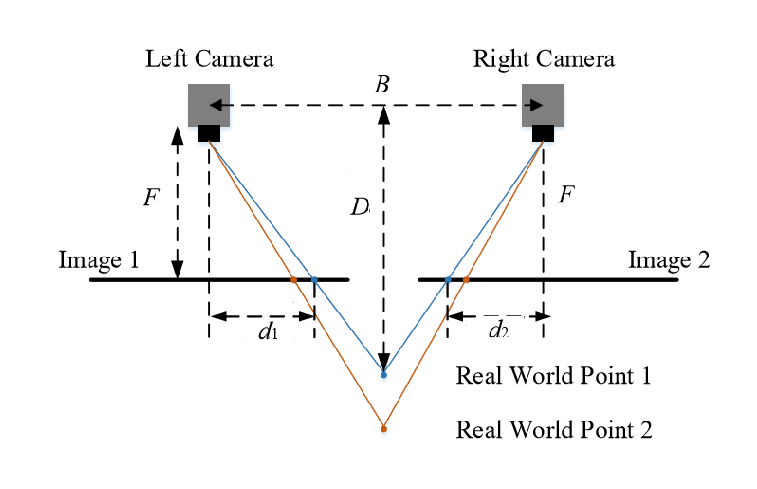
\includegraphics[keepaspectratio]{Principle-of-stereo-cameras.png}}
\caption{Stereo camera}
\end{figure}

\textbf{Figure 3:} Using cameras that are a known fixed ttransformation
apart, depth in the scene can be estimated using the difference in the
image produced by the two sensors.\{==cite==\}

The projection matrix of the camera that we are using in this project is
found to be:

\[\mathbf{K} = \begin{bmatrix} 595.998 & 0 & 320.825 \\
0 & 595.998 &239.252 \\
0 & 0 &1\end{bmatrix} \]

Methodology

In our project, we propose to use a vision based system to develop
perception algorithms for DSO. We introduce the different hardware and
software aspects of the proposed perception algorithm.

\begin{figure}
\centering
\pandocbounded{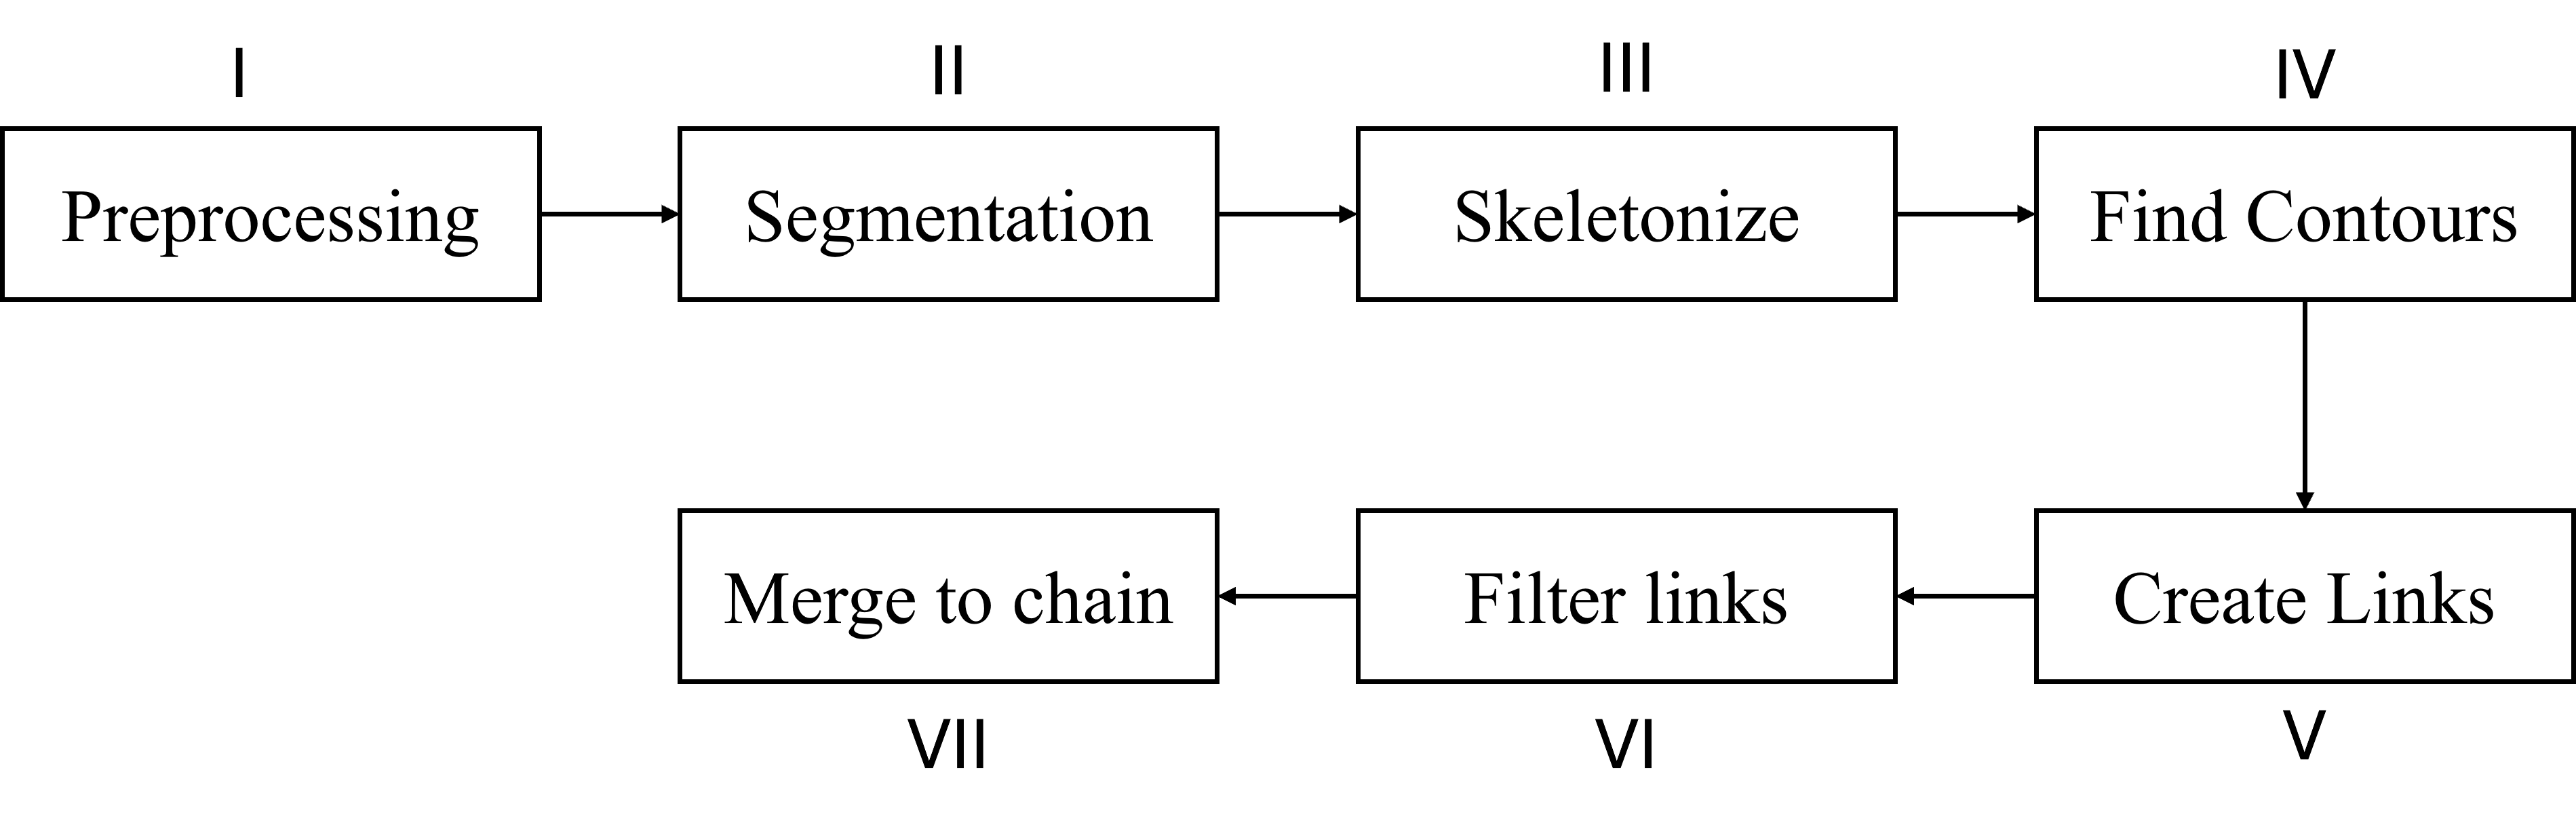
\includegraphics[keepaspectratio]{Methodology.png}}
\caption{Software methodology}
\end{figure}

\textbf{Figure 4:} The steps taken in this methodology

\subsection{I. Preprocessing}\label{i.-preprocessing}

The RGB-D data obtained from the camera is preprocessed to downsample it
to a standard size of \(640\times 480\). Further the image is filtered
with gaussian blurring to smooth out the image for noise. A gaussian
kernal of \{==size==\}

\begin{figure}
\centering
\pandocbounded{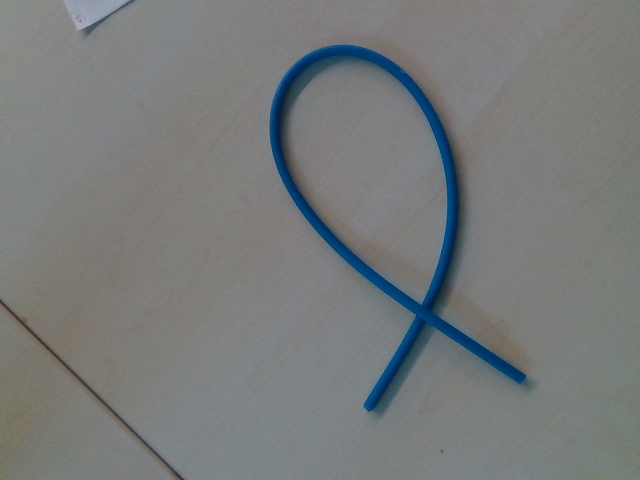
\includegraphics[keepaspectratio]{example_image.png}}
\caption{Preprocessed\_image}
\end{figure}

\textbf{Figure 5:} A typical example of an image of the DSO being
manipulated

\subsection{II. Segmentation}\label{ii.-segmentation}

The stereo camera will give us dense data about all the pixels in the
image. However, in most cases, we only need certain sparse data that
pertains to our problem. In this case, we only need RGB-D data of the
deformable slender object that we will be manipulating. To achieve this,
we use segmentation to find which pixels in the image correspond to the
DSO. Image segmentation is the process of splitting an image into
different sets of pixels based on some condition. There are different
methods of doing image segmentation:

\begin{itemize}
\tightlist
\item
  \textbf{Semantic segmentation}: Classifies the pixels based on the
  meaning of the object. Employs deep learning methods that can learn
  the pixel based classification problem. Example U-net
\item
  \textbf{Region-based segmentation}: Classifies the pixels based on
  similarities between nearby pixels. The criteria for similarity can be
  color, texture etc.
\end{itemize}

\subsubsection{Semantic segmentation}\label{semantic-segmentation}

Semantic segmentation is typically done using deep-learning models. They
have the ability to learn the meaning behind the image and therefore
successfully classify the pixels that belong to a certain kind of
object. The deep learning models that do this have an autoencoder
architecture. Unet is a highly successful model that employs skip
connections that ensures that finer details of the image can be
successfully classified. To train the network for semantic segmenations,
we need to have poxel wise labels for each image in the training data.
The training is done to minimise the focal loss for each pixel.

\begin{figure}
\centering
\pandocbounded{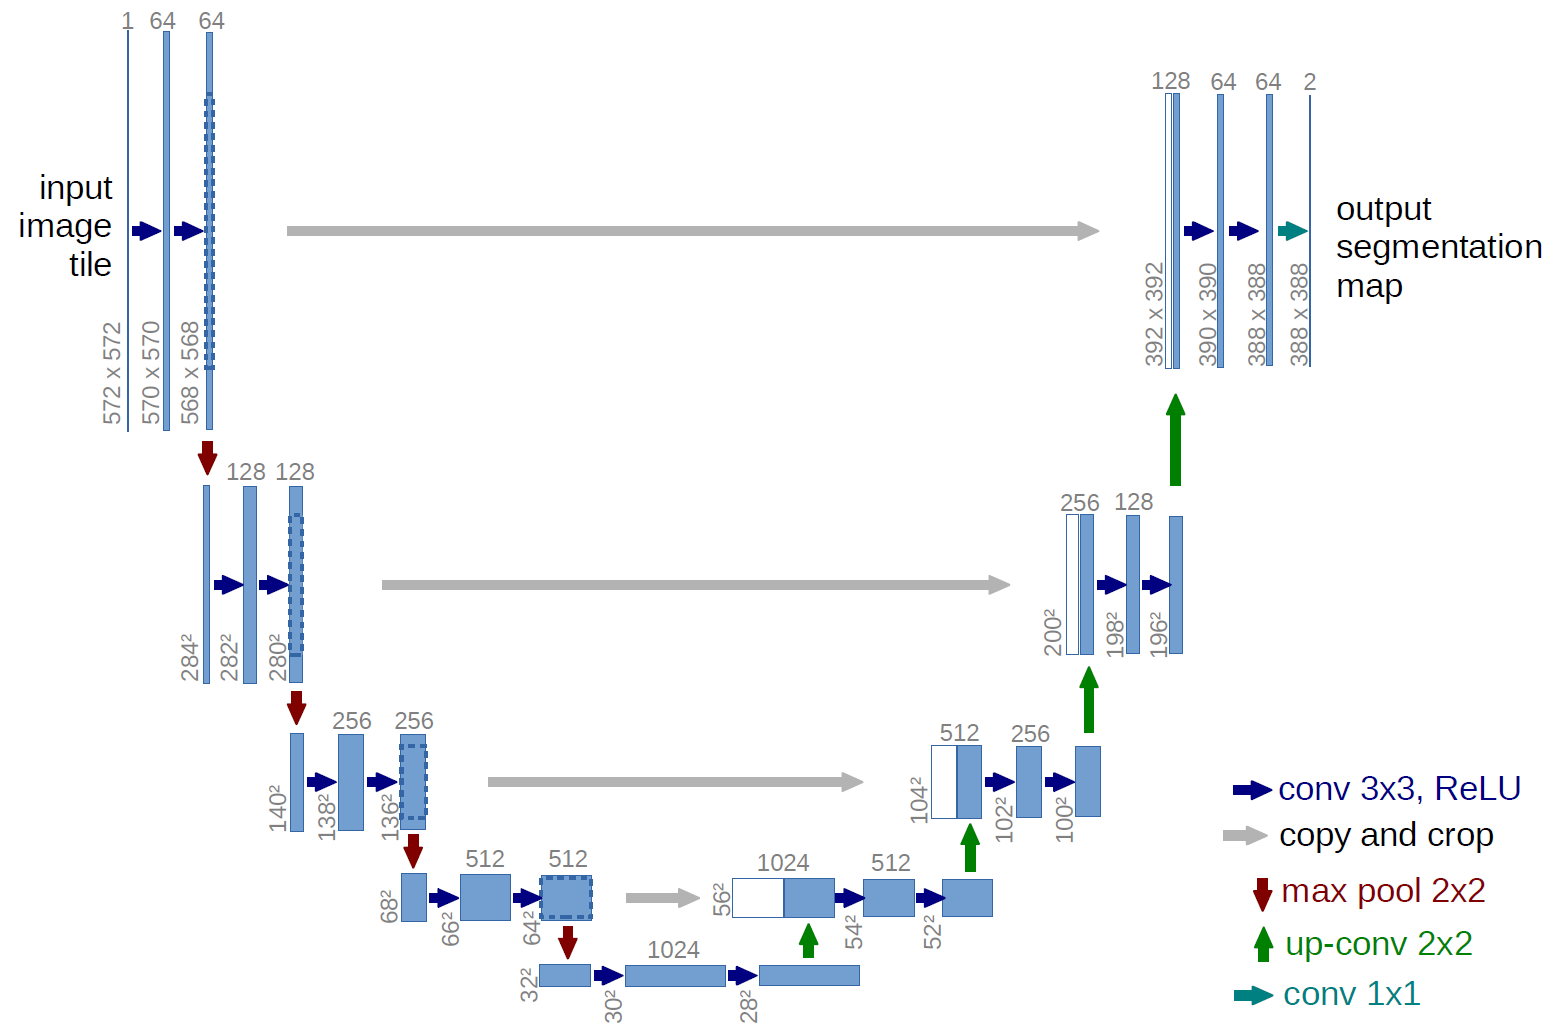
\includegraphics[keepaspectratio]{u-net-architecture.png}}
\caption{alt text}
\end{figure}

\textbf{Figure 6:} Deep-learning based semantic segmentation model.

Semantic segmenation requires large amounts of data to give accurate
results. There are other methods of segmentation that can be used to
segment the deformable slender object from the image.

\subsubsection{Region-based
segmentation}\label{region-based-segmentation}

Segmentation can also be performed based on other aspects of the image.
For example, a group of pixels having the same color or texture can be
segmented. In this project, we adopt color based segmentation to find
the pixels that are associated with the DSO. For color-based
segmentation, we convert the RGB image into the HSV color space because
it is less dependant on lighting conditions. In our case, the DSO is
blue in color, so we set the limits in the HSV Space as:

\textbackslash{[}\mathrm{Lower limit} =
{[}100,150,50{]}\textbackslash{]} \textbackslash{[}\mathrm{Upper limit}
= {[}140, 255, 255{]}\textbackslash{]}

All the pixels that do not belong in this interval are equated to zero.

\begin{figure}
\centering
\pandocbounded{\includegraphics[keepaspectratio]{hsvcone.gif}}
\caption{HSV\_color\_space}
\end{figure}

\textbf{Figure 7:} HSV color spaced used for color based segmentation

\begin{figure}
\centering
\pandocbounded{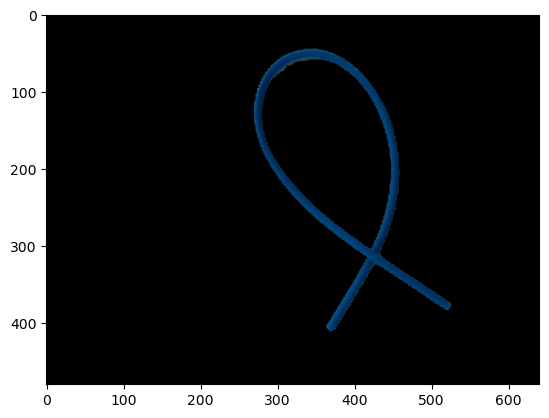
\includegraphics[keepaspectratio]{segmented_image.png}}
\caption{Segmented\_image}
\end{figure}

\textbf{Figure 8:} Example image after color based segmentation

\subsection{III. Our method}\label{iii.-our-method}

To obtain the topology of the DSO from the image, we construct the
skeloton of the image using Zhang's method {[}@Zhang1984{]}. Zhang's
Method for skeletonization is an efficient algorithm for thinning a
binary image to obtain a skeleton representation of shapes. The method
is based on iteratively removing pixels from the boundaries of the
objects in the binary image while preserving the topology and structure
of the shapes. Zhang's algorithm works by applying a series of
conditional rules that allow the removal of boundary pixels in a way
that retains the essential structure of the object. Specifically, it
works by iterating through the image and checking each pixel's
neighborhood for continuity, and then removing pixels that satisfy the
continuity. This process continues until no further pixels can be
removed, resulting in a skeleton that represents the object as a thin,
one-pixel-wide line.

\begin{figure}
\centering
\pandocbounded{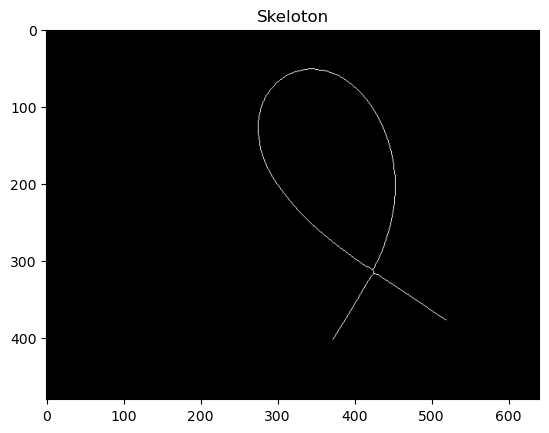
\includegraphics[keepaspectratio]{skeleton.png}}
\caption{Skelotonized}
\end{figure}

\textbf{Figure 9:} 1 pixel width representation of the rope

Now that we have a one dimensional representation of the DSO in the
image plane, we can find the contours that represent the topology of the
DSO. Contours are a sequence of points on the skeleton that are
continous. When occlusions occur, the image of the rope might not be
continous and we may have several disjoint contours. Moreover, when
there are self-occlusions, the contour might not follow the actual
direction of the DSO an example of this is shown in:
\pandocbounded{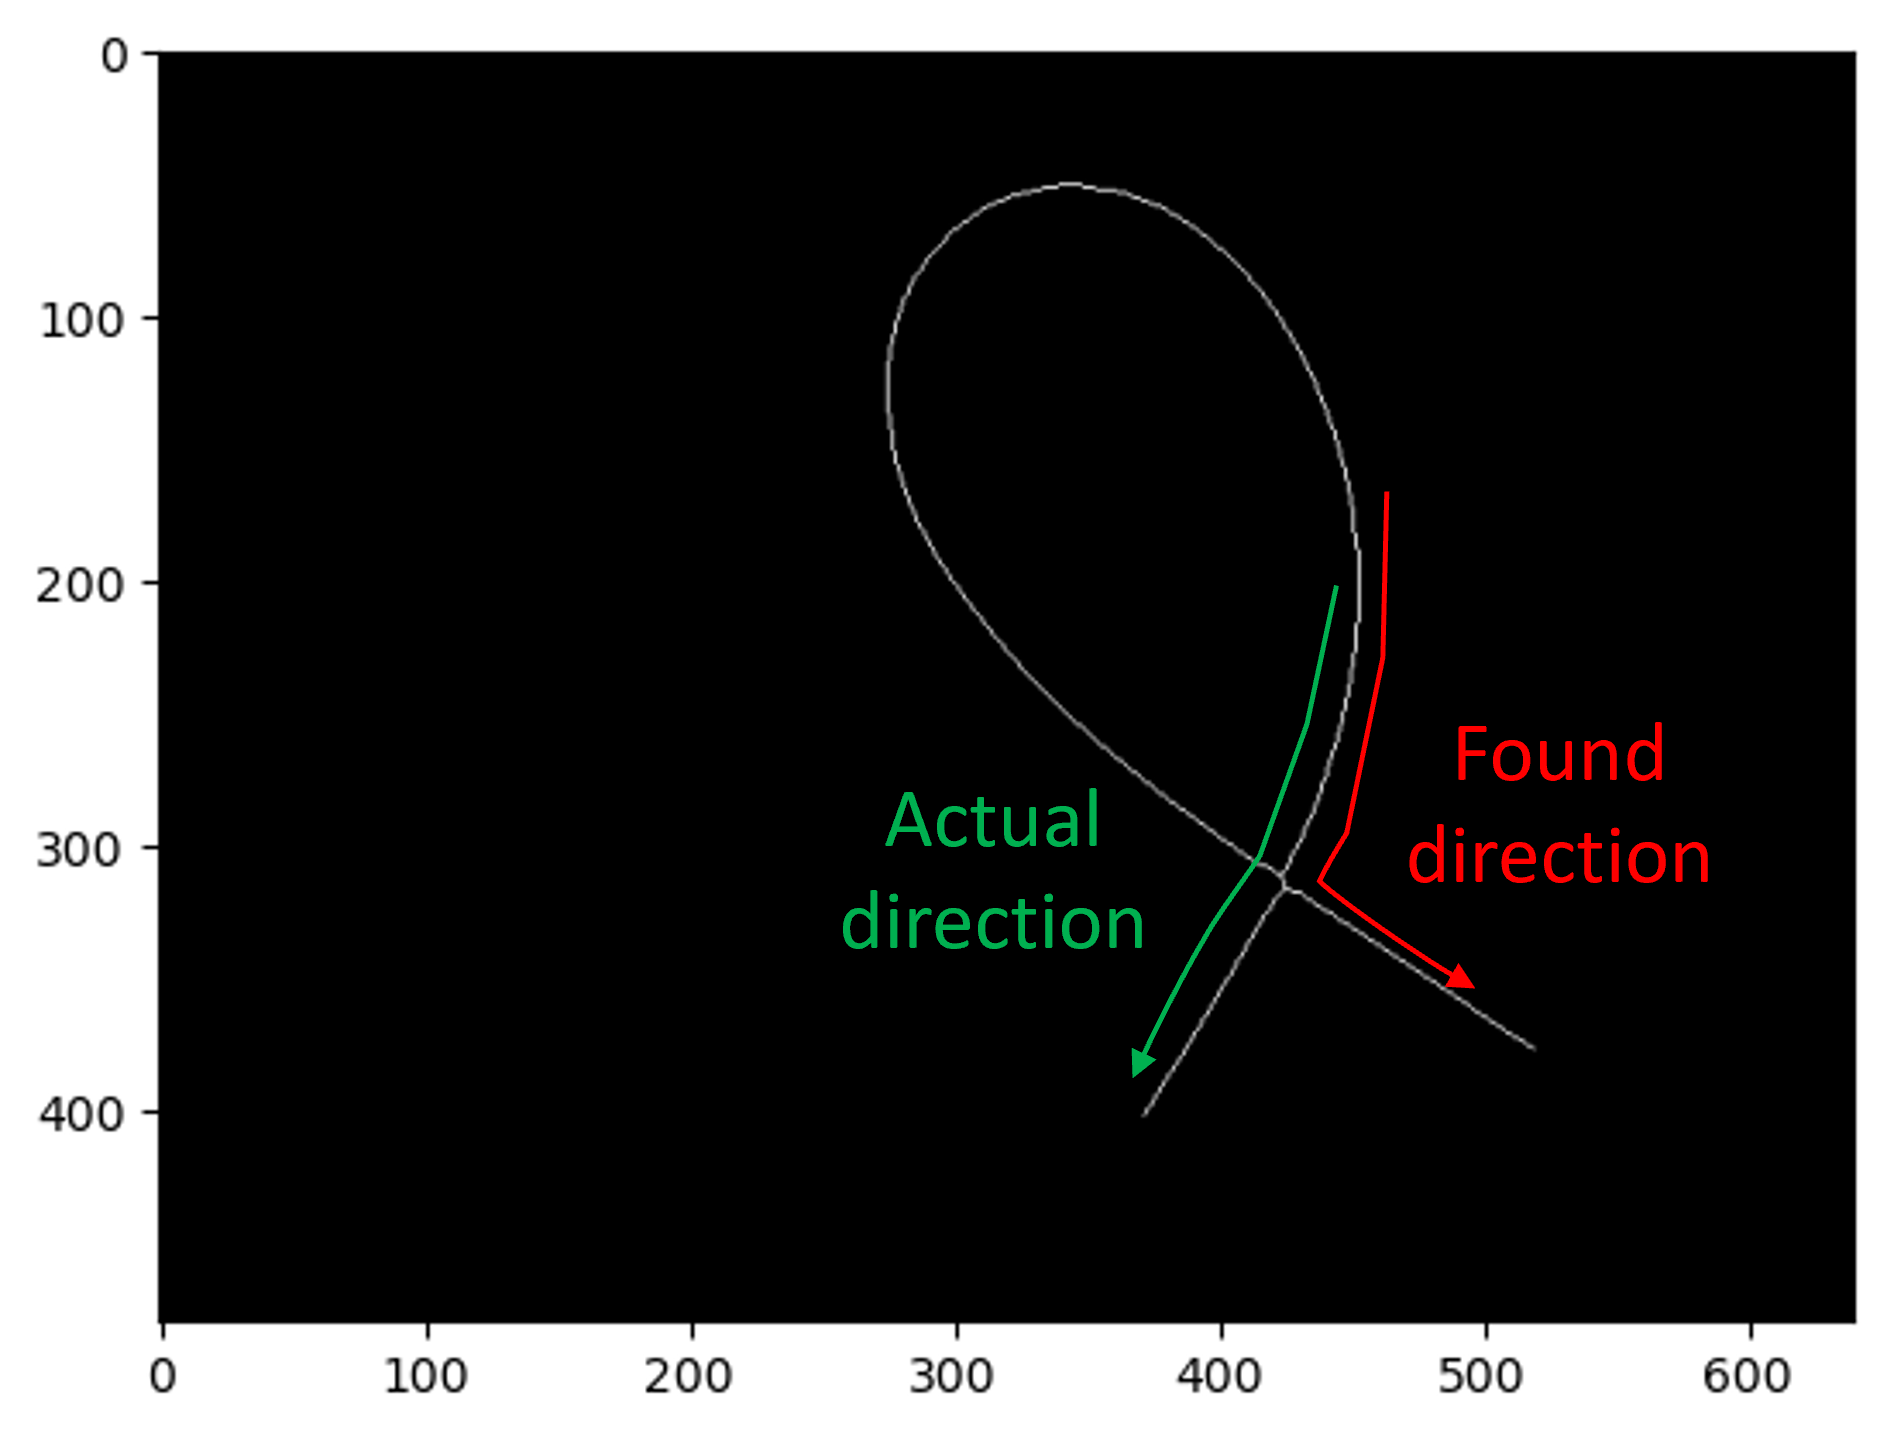
\includegraphics[keepaspectratio]{Contours.png}}

To overcome this problem, we design an algorithm that operates on
smaller segments of each contour to identify locally linear chains of
connected points. For each contours, it traverses the points
sequentially and splits it into smaller segments based on the local
curvature. The traversal begins by initiallizing a starting point for
the current segment. As points are added, the algorithm checks whether
the euclidean distance between the segment starting point and the
current point exceeds a fixed segment length \(l_{thresh}\). If this
length threshold is reached, the direction of the current segment is
calculated using \(\theta_i = (x_s - x_i,y_s - y_i)\) where
\((x_s,y_s)\) and \((x_i, y_i)\) are the positions of the start of the
segment and the current point in the image plane. If the angle between
the current and the previous segment is below a predefined threshold
\(\theta_{thresh}>= \theta_i \cdot \theta_{i-1}\), this segment is added
to the chain. Otherwise, a new chain is initialized. Through this
method, we obtain a set of chains that are spacially coherant.

\begin{figure}
\centering
\pandocbounded{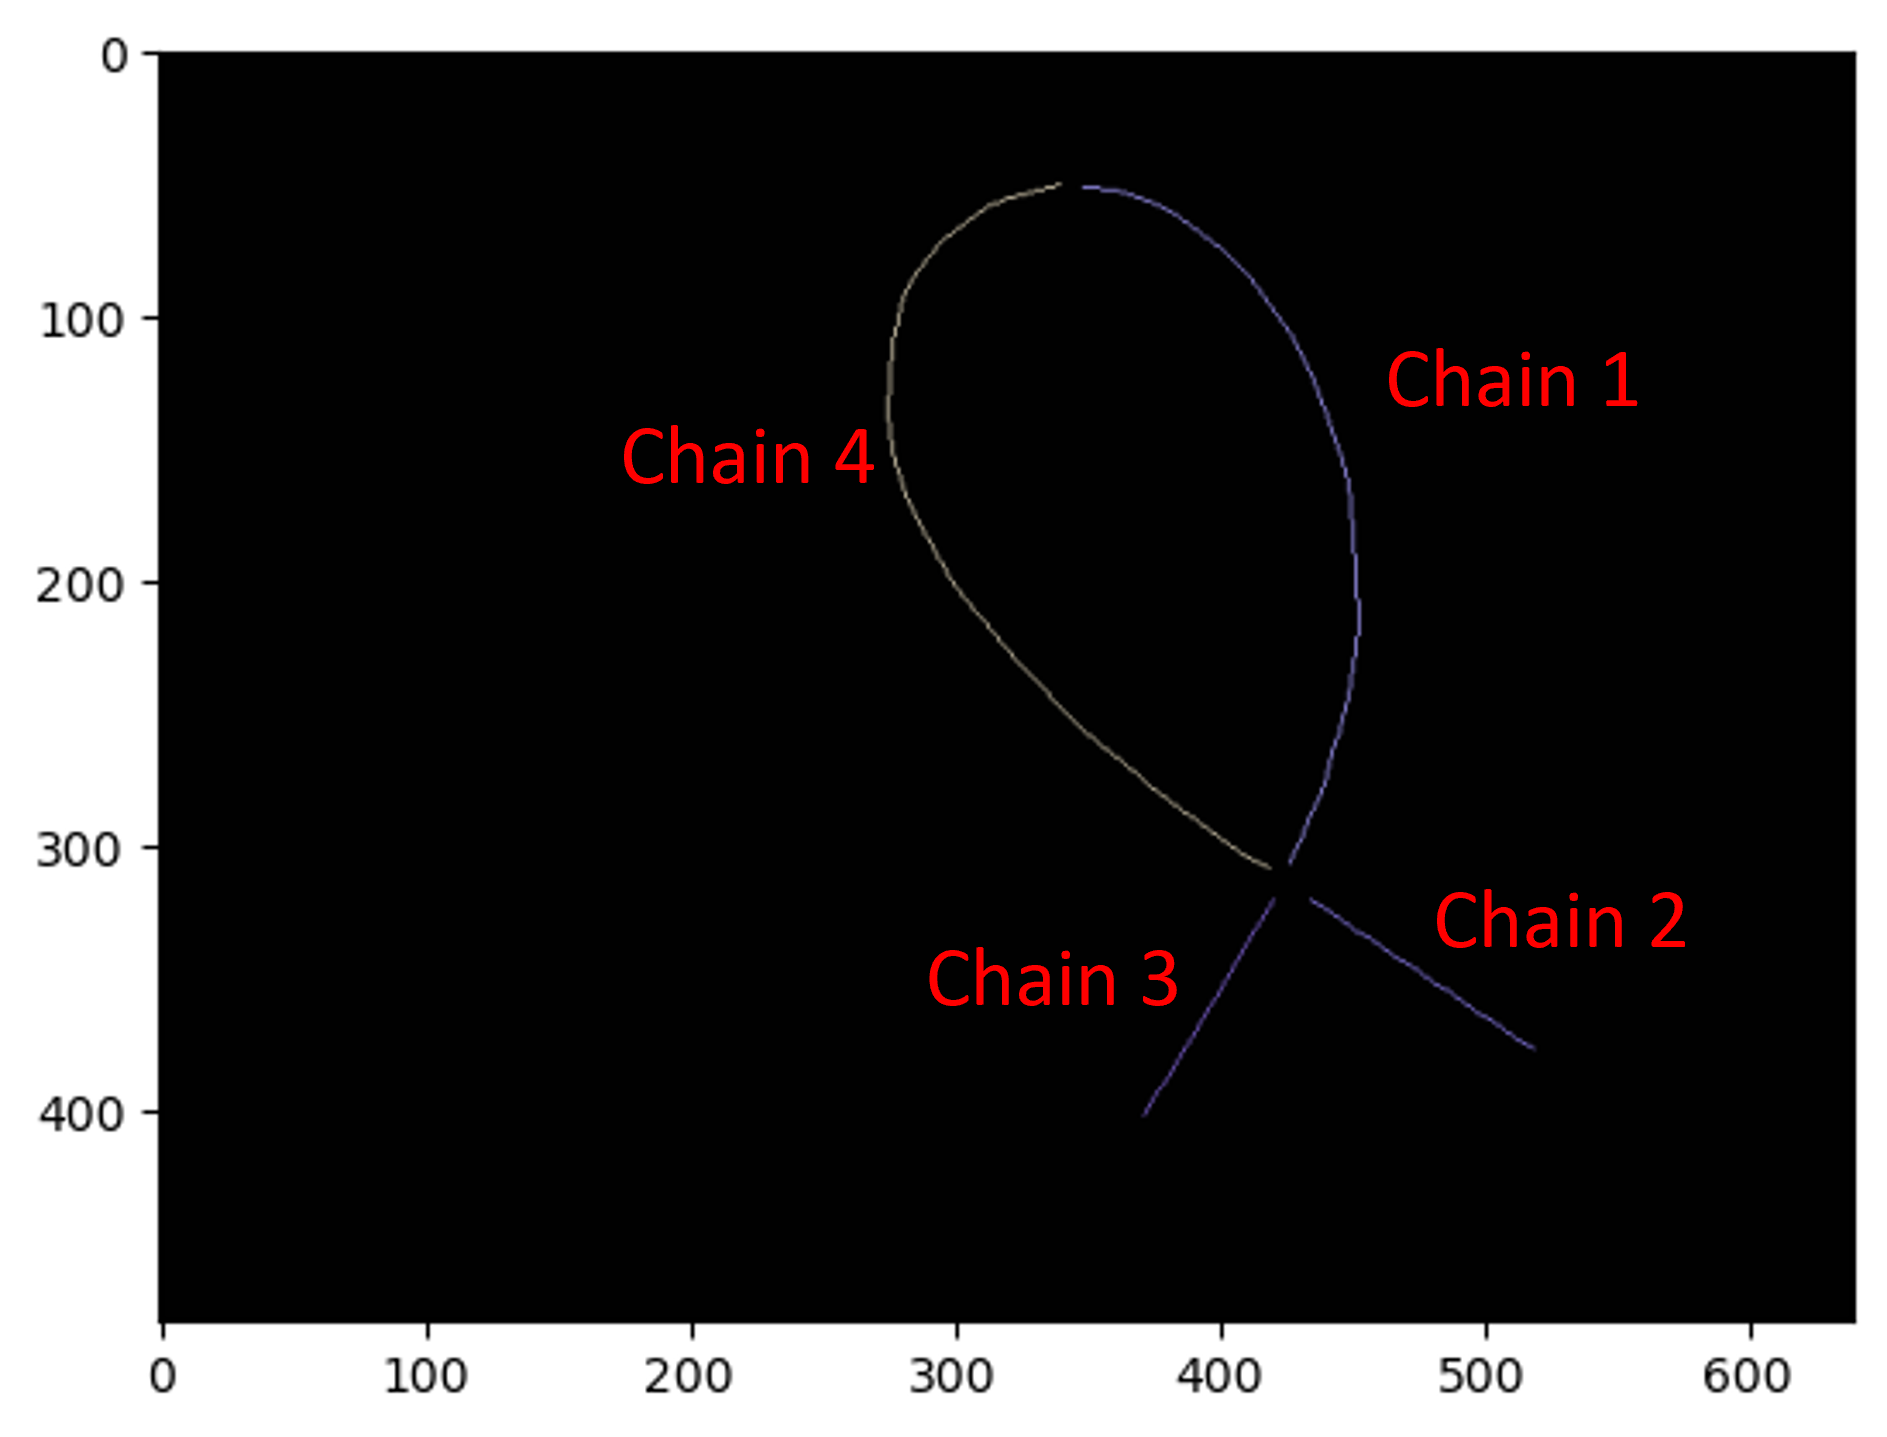
\includegraphics[keepaspectratio]{chains.png}}
\caption{image}
\end{figure}

\textbf{Figure 1:} The different chains created from the contours of the
DSO skeleton.

The disjoint chains should now be rejoined to form the sequence of
points that form the skeleton of the DSO. Each chain has two ends, so
for an image that has \(n\) chains, the total number of ends will be
\(2n\). The number of possible combinations are \(\frac{n(n-2)}{2}\). To
decide how the combination of chains should be, we use the hungarian
algorithm which requires a cost matrix \(\mathbf{C}\) that determines
the cost of every possible assignment. The hangarian algorithm tries to
minimise the cost function:

{[}\min \sum\_\{k=1\}\^{}\{2n\} \mathbf{C}(k,\sigma(k)){]}

where \(\sigma(i)\) is the end of the chain that is assigned to the end
at \(i\). The cost associated with connecting end \(k\) with end \(l\)
is computed as a combination of the curvature \(C_c(k,l)\) and the
euclidean distance \$C\_e(k,l).

{[}C(k,l) = \lambda\_e C\_e(k,l) +\lambda\_c C\_c(k,l){]}

{[}C\_\{k,l\} = \lambda\_e \sqrt{(p_k - p_{l})^2} + \lambda\_c
\left(\cos\^{}\{-1\}\left(\frac{(p_k-p_l)\cdot p'_k}{\|(p_k-p_l)\| \|p'_k\|}\right)
+
\cos\^{}\{-1\}\left(\frac{(p_k-p_l)\cdot p'_l}{\|(p_k-p_l)\| \|p'_l\|}\right)\right){]}

The euclidean norm ensures that the two endds are close to each other
and the curvature cost will ensure that joining them together will not
cause a sharp change in the direction of the rope. We also have a few
special cases that must be accounted for such as one end of a chain is
not allowed to be joined with itself. To discourage this, we populate
the diagonal elements of the cost matrix with large numbers, in this
case it is chosen to be \(10^5\). The values of the diagonal elements
and the weightage for euclidean and curvature cost is found through
trial and error to see which provides the best performance. The final
weightage that we used are \(\lambda_e = 0.001\) and \(\lambda_c = 1\)

\begin{figure}
\centering
\pandocbounded{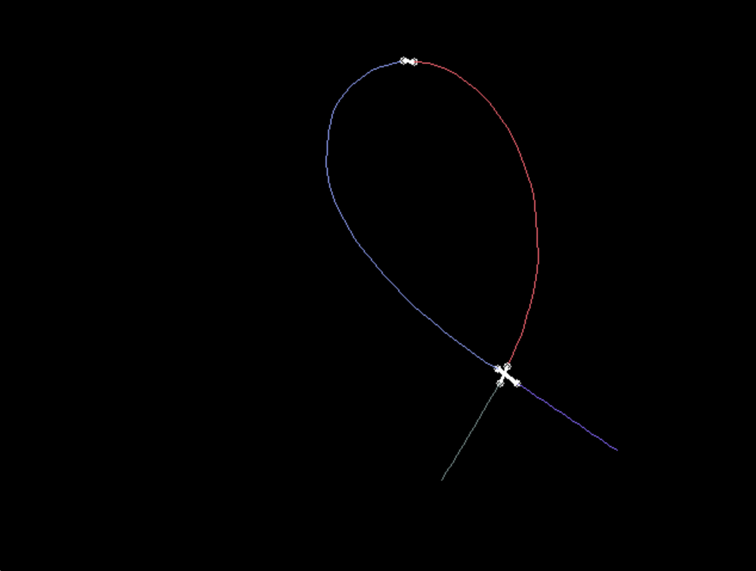
\includegraphics[keepaspectratio]{image-1.png}}
\caption{alt text}
\end{figure}

\textbf{Figure 1:} The disjoint chains are connected based on the
solution of the hungarian algorithm.

\pandocbounded{\includegraphics[keepaspectratio]{Algorithm_video.mp4}}\{`width:
40\%'\}

\textbf{Video 1:} Overview of the image processing

\subsection{3D reconstruction}\label{d-reconstruction}

Using the depth data at the points where the rope exists, we can
reconstruct the shape of the rope in 3D. This is done by first inverting
the perspective projection through:

{[}\mathbf{P}\_x = \frac{(\mathbf{p}_x - c_x)}{f_x} \mathbf{P}\_z{]}

{[}\mathbf{P}\_y = \frac{(\mathbf{p}_y - c_y)}{f_y} \mathbf{P}\_z{]}

The z-cordinate can be obtained directly from the depth image
corresponding to \(p_x\) and \(p_y\). Using this, we can approximate the
3D shape of the DSO.

Figure 1: Overview of the image processing

Given an image of the rope taken from an RGB-D camera, we can use the
spatial relationship between different parts of the DSO to obtain a
coherent 3D representation of the DSO. However, during occlusions, we
have missing parts of the DSO and disjointsections of the DSO in the
image. To account for the occlusions, we also make use of some temporal
dependencies.

\section{Temporal dependencies}\label{temporal-dependencies}

The evolution of the DSO under manipulation will follow the dynamics of
the DSO. This depends on the matrial parameters, the external and
internal forces on the DSO. The external forces include gravity,
manipulation forces and contact with other objects in the environment.
On the other hand, the internal forces could arise from the objects
elastisity, damping etc. Some of the forces, like gravity, can be easy
to measure, however, internal forces or forces from contact with the
environment may be difficult to measure from an experiment. Therefore,
we do not use the full dynamics of the DSO, rather we make the
assumption that the dynamics of the DSO is a smooth and continous. We
can use the assumption of smoothness to identify the shape of the DSO
under occlusion where we cannot directly measure the DSO position using
the camera. There can be many different approaches to leveraging this
assumption. In this project, we make use of smoothing splines to obtain
a smooth representation of the DSO shape that remove outliers and fill
missing information.

To leverage the temporal dependencies, we use a video obtained of the
manipulation of the DSO. Using the spacial dependence, we obtaine
\((x(t), y(t), z(t))\) for various points on the DSO throughout the
manipulation time. We fit 3rd order splines with a smoothing factor of
0.5 for \(x(t)\), \(y(t)\) and \(z(t)\). The spline is then used to find
missing data due to occlusions. Using this method, we are able to
estimate the shape of the DSO even when it is occlusded by a
manipulator.

Results

To test our methodolgy of making segmentation of DSOs aware of
occlusions that may be unavaoidable during manipulation, we choose a
slender object that can be used as the object for manipulation. To
simplify our experiments, we choose the manipulate the DSO with our
hands rather than using a robotic manipulator. Although our end-goal is
for this method to be used for robotic manipulation, we can use hand
manipulation because the problems like occlusions will still be present
in hand manipulation.

We initialize the experiment by placing the DSO on a table such that
there are no occlusions of the DSO. We record a video of the DSO while
we move the DSO such that there are occlusions due to our hand as well
as due to other parts of the DSO itself. We investigate the performance
of our method firstly by only considering the spacial dependenciesof the
DSO. We then investigate how the results change when we incorporate the
temporal dependencies as well. The video of the DSO manipulation
conducted is shown

\pandocbounded{\includegraphics[keepaspectratio]{experiment.mp4}}\{`width:
40\%'\}

\textbf{Video 2:} Manipulation of the DSO

Explointing the spacial dependencies only, we attempt to find the 3D
reconstruction of the DLO during manipulation. The reconstruction
throughout the manipulation experiment is shown in video

\pandocbounded{\includegraphics[keepaspectratio]{spacial.mp4}}\{`width:
40\%'\}

\textbf{Video 4:} When there are inevitable occlusions of the DSO by the
manipulator. There are missing points on the DSO image.

Now using the temporal dependancies, we can create a more accurate
reconstruction of the manipulated object

\pandocbounded{\includegraphics[keepaspectratio]{temporal.mp4}}\{`width:
40\%'\}

\textbf{Video 4:} When there are inevitable occlusions of the DSO by the
manipulator. There are missing points on the DSO image.

\section{References}\label{references}

{[}1{]} M. Saha and P. Isto, ``Manipulation planning for deformable
linear objects,'' IEEE Transactions on Robotics, vol.~23, no. 6,
pp.~1141--1150, 2007.
